El problema general de estimación consiste en dado un modelo de observación,
\begin{equation}
	y=f(\x,\eta)
\end{equation}
estimar $x \in \R(n)$ de las observaciones $y \in \R(m)$ donde $\eta$ es una perturbación desconocida y $f$ es una función de \textit{mapeo} que determina el modelo).

El problema de la estimación es de gran interés y extensivamente investigado en diferentes campos de aplicación del control y el procesamiento de señales \cite{Ruiz2009}.
Dependiendo de si el modelo del entorno $f$ es lineal o no lineal, los métodos de estimación varían considerablemente. 
Generalmente se utilizan para el primer caso, técnicas de estimación lineales o linealizadas de una sucesión de datos.
Si $f$ es lineal, se puede expresar de la forma,
\begin{equation}
	\z=\mH \x+\mB \eta
\end{equation}
donde, $\mA$ define la relación lineal entre el parámetro desconocido $\x$ y la observación realizada $\y$;
$\mB$ representa el modelo completo de perturbaciones del sistema. Este tipo de problemas lineales se resuelve mediante la  estimación de mínimos cuadrados (LMS \ing{Least mean squares}).\par
%Hay razones para creer que algunos elementos de las observación son de mas confianza que otros y pueden contribuir mejor a la estimación final. Es posible modificar la LMS incluyendo una matriz de pesos diagonal $W$
%para la discriminación de las observaciones. %Form10 Form11
%El método de la máxima verosimilitud (MLE) utiliza un modelo de las características del ruido del sistema.\\
%También es posible definir si hay valores que \textit{a priori} son más probables que otros, mediante la obtención de la caracterización estadística \textit{a priori} de la variable desconocida $x$.\\
La mayoría de los métodos de fusión sensorial se basan en la regla de Bayes para la combinación de información \textit{a priori} del estado del sistema y las observaciones.
La regla de Bayes provee un medio para hacer inferencias acerca de un objeto u entorno de interés descrito por un estado $x$, dada una observación $y$.
Mediante la inferencia bayesiana se establece la relación entre $x$ y la medición $y$, mediante una probabilidad conjunta para variables discretas, o una PDF conjunta, $P(x,y)$ para variables aleatorias continuas.
Si se conoce la función de densidad de probabilidad (PDF) de $x$ con anterioridad, $p(x)$, es posible utilizar los estados del teorema de Bayes,
\begin{equation}
	P(x|y)=\frac{P(y|x)P(x)}{P(y)}=\frac{P(y|x)P(x)}{\int{P(y|x)P(x)dx}}
\end{equation}
$P(y|x)$ cumple el rol de un modelo de sensor.
Para cada valor de $x$, se define una probabilidad en $Y$.
El argumento para máximo de una probabilidad \textit{a posteriori} estima el valor de $\hat{x}$.\par
El problema de filtrado es un caso particular del problema de estimación generalizado.
El cual consiste en inferir en cada instante el valor de una señal interna de un sistema dinámico, controlado por entradas conocidas y desconocidas,
utilizando muestras de entradas y salidas presentes y pasadas.


\subsection{El filtro de Kalman}
\label{subsec:kalmanfilter}
%Filtro de Estimador lineal recursivo que calcula y estima para valores de estado continuos, basándose en obsercaciones periódicas de el estado
No siempre es posible observar y medir todos los estados de un sistema,
por tal motivo se hace necesario realizar estimaciones de estos a partir de mediciones proporcionadas por sistemas de sensado ruidoso.
Tal cual como se observa en la figura~\ref{filtproblem}.
Es posible realizar un modelo probabilístico del sistema mediante la implementación de filtrado bayesiano.
El KF un caso particular de un filtro bayesiano recursivo cuando las densidades de probabilidad de los estados del entorno son todas gaussianas.
\onePic{filtproblem}{Representación del problema general del filtrado. Donde $S$ es un operador que mapea las señales de entrada $u$ y $w$, en las señales de salida $v$ y $y$.}{Ruiz2009}{0.7}
EL filtro de Kalman es un estimador óptimo recursivo de mínimos cuadrados,
basado en los cálculos de la media condicional y la covarianza de la distribución de la probabilidad del estado del sistema.
El filtrado de Kalman se utiliza con el fin de reducir los efectos causados por el ruido del sistema y de medida, también para poder estimar estados no observables por una no disponibilidad de los sensores o la imposibilidad de su instalación.
%mediante la iteración de etapas de predicción y estimación.
El filtro establece un modelo estadístico explicito de como un conjunto de observaciones $\mathbf{z}$ están relacionadas a los parámetro de estado  $\mathbf{x}$ \cite{Bar-Shalom2002}, \cite{Toledo-Moreo2007}.\par
El filtro de Kalman tiene muchas ventajas que le permiten realizar estimación mediante fusión multisensorial y resolver problemas complejos de esta índole.
El filtro funciona bien donde es posible determinar las observaciones y los modelos dinámicos de transición del sistema.
%, es decir donde están bien definidas las descripciones de los estados.
El filtro utilizado para sistemas lineales e iteraciones discretas en el tiempo es el filtro de Kalman-Bucy \cite{Kalman1960},\cite{Kalman1961}.\par
Es necesario definir un modelo para los estados a estimar en la forma estado-espacio estándar considerando los siguientes modelos de series de tiempo,
\begin{align}
	\mathbf{x}_{k+1}&=\mA \mathbf{x}_k + \mathbf{w}_k\\
	\mathbf{z}_{k}&=\mH \mathbf{x}_k + \mathbf{\eta}_k
\end{align}
Donde, $\mA$ es la matriz de transición de estados;
$\mH$ es la matriz que relaciona las observaciones con el estado actual
y $\mathbf{w}_k$ y $\mathbf{\eta}_k$ son ruidos de procesos y de medición respectivamente.
Estas ecuaciones definen la evolución de un sistema de tiempo continuo con observaciones continuas hechas sobre el estado.
Conociendo una observación $\mathbf{z}_{k}$ es posible encontrar y actualizar la estimación de $\mathbf{x}_{k+1}$.
%La solución es una combinación lineal de dos variables aleatorias gaussianas. El resultado también  es una variable aleatoria gaussiana.
El algoritmo de filtrado de Kalman produce estimaciones que minimizan el error medio cuadrado de la estimación gracias a la fusión de sensores de vector de observación $\mathbf{z}_{k}$.
Los diagrama de flujo del filtro Kalman se encuentra en la figura \ref{KF}.\par
\begin{figure}[h!]
	\centering
	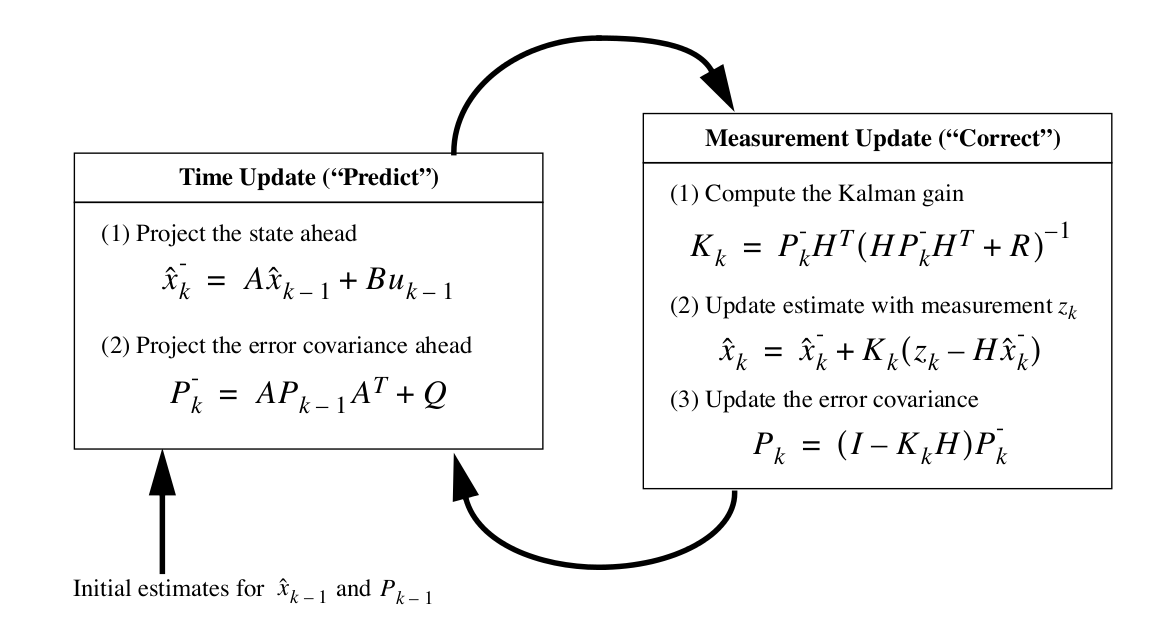
\includegraphics[width=0.8\columnwidth]{KF}
	\caption{Diagrama del filtro de Kalman}
	\label{KF}
\end{figure}

En la gráfica~\ref{KF}, $P_{k}$ es la covarianza del error asociada a la estimación (en predicción o correción) en el momento $k$;
$Q_k=E[w_k w_k^\intercal]$ y $R_k=E[v_k v_k^\intercal]$ son las matrices de covarianza de los ruidos de proceso y medición respectivamente.
Este filtro funciona muy bien para sistemas que se asumen lineales.
Si el el sistema es no lineal, es necesario realizar algún tipo de aproximación o modificación de este.
Si es necesario realizar técnicas de estimación no lineal para datos secuenciales,
los modelos de las perturbaciones continúan siendo aditivos, pero los modelos del sistema contienen elementos no lineales y el modelo de estado se denota como un espacio de estado con una ecuación vectorial diferencial no lineal de primer orden,

\begin{align}
	\mathbf{x}_{k+1}&=f(\mathbf{x}_k) + \mathbf{w}_k\\
	\mathbf{z}_{k}&=g(\mathbf{x}_k) + \mathbf{\eta}_k
\end{align}

Para resolver este sistema es posible utilizar una variación especial del Filtro de Kalman denominada filtro de Kalman Extendido (EKF).
El EKF linealiza el sistema alrededor de un punto y estado de operación $\x_k$.
Que es muy parecido en su desarrollo al mismo filtro de Kalman, 
funcionando bajo un esquema de predicción y actualización, pero utiliza series de expansión de Taylor para linealizar los elementos no lineales de las estimaciones.

Los diagrama de flujo del filtro Kalman extendido se encuentra en la figura \ref{EKF}. 
\begin{figure}[h!]
	\centering
	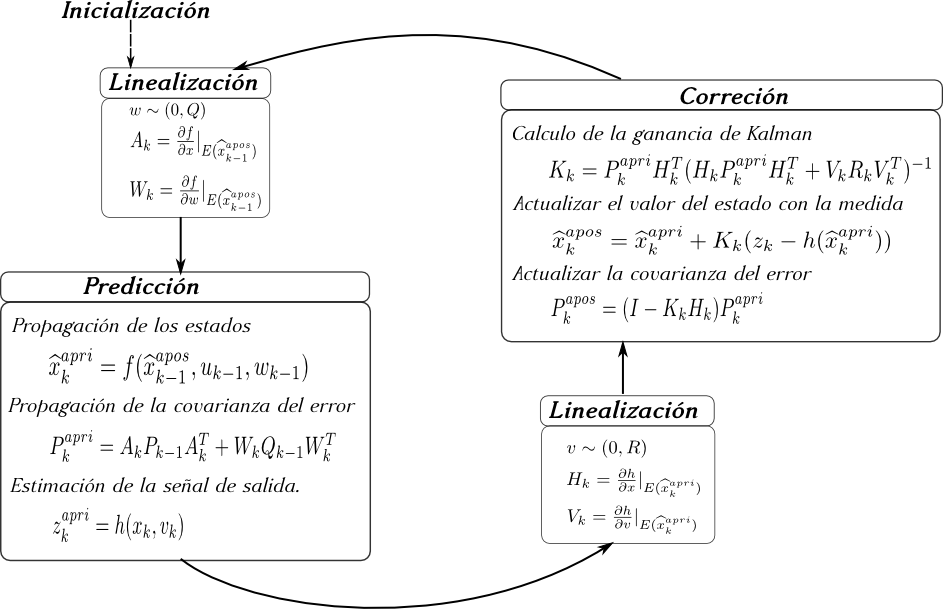
\includegraphics[width=0.9\columnwidth]{EKF}
	\caption{Diagrama del filtro de Kalman extendido.}
	\label{EKF}
\end{figure}
%
%Donde,
%$E[\alpha]$ valor esperado de $\alpha$
%$A_k$ valor de la cunción $A$ en el momento $t_k$
%$x_{k|l}$ refiere al valor de $x$ en el tiempo $t_k$ dada medidas asociadas al tiempo $t_l$
%$\hat{x}$ estimación sw $x$
%$\bar{x}_0$ estimación a priori de $x_0$, que es la estimación de $x_0$ sin haber recibido mediciones.
%Si se asume concoimiento priori el algoritmo es igual al filtro de Kalman
%dado $\bar{x}_0$
%$P_0=E[(x-\bar{x}_0)(x-\bar{x}_0)^\intercal]$
%Se asume que la entrada $u_k$ es conocida.
Durante la aproximación del filtro EKF se utilizan las siguientes linealizaciones,
\begin{equation}
	\mA_k=\pdv{\mF(\x,\u)}{\x^\intercal} \vline_{\x=\x_k,\,\u=\u_k}
\end{equation}

\begin{equation}
	\mH_k=\pdv{h(\x)}{\x^\intercal} \vline_{\x=\x_k}
\end{equation}

Para cada instante se calcula la ganancia del filtro $L$ y se actualiza la estimación del estado y la matriz de covarianza
\begin{equation}
\begin{array}{rcl}
\mL_k&=&\mP_{k|k-1} \mC_k^\intercal [\mC_k \mP_{k|k-1}\mC_k^\intercal + \mR_k]^{-1}\\
\hat{\x}_{k|k}&=&\hat{\x}_{k|k-1} + \mL_k (\z_k-h(\hat{\x}_{k|k-1}))\\
\mP_{k|k}&=&\mP_{k|k-1} - \mL_k \mC_k \mP_{k|k-1}
\end{array}
\end{equation}

La propagación de la estimación de el estado y la matriz de covarianza en el siguiente instante de medición se encuentra mediante,
\begin{equation}
\begin{array}{rcl}
\hat{\x}_{k+1|k}&=&\mF(\hat{\x}_k,\u_k)\\
\mP_{k+1|k}&=&\mA_k \mP_{k|k} \mA_k^\intercal + \mG_k \mQ_k \mG_k^\intercal\\
\dot{\hat{\x}}&=&\mA\hat{\x}+\mB\u+\mK(\z-\mC\x)
\end{array}
\end{equation}

Este filtro se utilizó en el simulador de filtrado de vehículo plano \ref{sec:simulator}.

\begin{comment}
%
%Si se denota 
%$e_k=\hat{x}_k-x_k$
%el error de la ecuación satisface la ecuación homogénea (propagación del error)
%$\dot{e}=(A-KC)e$
%Se sabe que si el sistema $(A,C)$ es observable, 
%podemos encoger una matriz de ganancia del observador tal que
%(A-KC) tiene un espectro de parte real negativa, esto implica que $e(t) \to 0$ cuando $t \to \infty$
%Luenberger (1966).
%La ganancia K se puede determinar mediante diferentes formas
%agregación de polos
%solución constante de una ecuación de Riccati
%Las ecuaciones de las mediciones estan dadas por
\begin{equation}\label{key}
\begin{array}{rcl}
H_x&=&x + \alpha \cos \hat{\theta}\\
H_y&=&y + \alpha \sin \hat{\theta}
\end{array}
\end{equation}
Encontrar el Jacobiano linealizado de la matriz de mediciones $H$, que se utiliza en la implementación del filtro de Kalman Extendido.
\begin{equation}
H_k=
\begin{bmatrix} 
\pdv{h_x}{x_k} & \pdv{h_x}{y_k} & \pdv{h_x}{\theta_k} \\
\pdv{h_y}{x_k} & \pdv{h_y}{y_k} & \pdv{h_y}{\theta_k} 
\end{bmatrix}
\end{equation}

donde n es el rango de la matriz de estado $A$
Para un sistema simple $[x,y,\theta]^\intercal$, $A$ es la matriz de identidad
\begin{equation}
x_{k+1}=
\begin{bmatrix} 
1&0&0\\
0&1&0\\
0&0&1
\end{bmatrix}
x_k+Bu_k
\end{equation}



%Form28
Otras aproximaciones a la estimación con los métodos de muestreo secuencial 
(sequential importance sampling),
los cuales son métodos de recurrencia bayesiana acumulativa, 
%El filtro de Kalman es un caso especial corrompido con ruido gaussiano
y donde los mas conocidos son los Filtros de partículas. %,consesancion, y otros
Funcionan mediante muestreado de las funciones de verosimilitud y del mismo sistema dinámico.
%Es posible muestrear de na función de verosimilitud p(yn|xn) y es posiboe muestrear de un modelo dimanimo p(xn|xn-1)
Son aplicables donde las técnicas de aproximación lineal no son suficientes y para problemas de una dimensión pequeña.\\
Los métodos secuenciales de Monte Carlo (MC) son métodos que describen las distribuciones de probabilidad como un conjunto de muestras ponderadas en un espacio de estado limitado. Se utilizan muestras para realizar inferencia probabilística mediante la regla de Bayes.
Los métodos MC se utilizan en problemas donde los modelos de transición entre estados y observaciones son altamente no lineales.
No se recomendable en problemas de muchas dimensiones, ya que el numero de muestras aumenta exponencialmente con las dimensiones de el espacio-estado.
Otra técnica utilizada para resolver problemas de linealidad es el filtrado de información, 
que se implementa de forma parecida al KF, pero en lugar de generar estimaciones de estado y covarianzas,
se utilizan variables de información de estado y matrices de información.
\begin{align}
\hat{y}(i|j)&=P^{-1}(i|j)\hat{x}(i|j)\\
Y(i|j)&=P^{-1}(i|j)
\end{align}
Tiene la misma estructura de predicción y actualización del KF, aunque la etapa de actualización es mucho mas simple de implementar.
El filtro de información se vuelve complejo para modelos no lineales por la dificultad en la extracción de la información.
Los filtros de Kalman e información se utilizan para problemas de fusión de datos donde las entidades de interés están bien definidas por un estado paramétrico continuo.
%El numero de partículas necesarias para dimensiones grande spuede ser exagerado
%Modelos graficos
La resolución de problemas de estimación mediante modelos gráficos,
permite representar relaciones dependencias en un conjunto de variables dentro de las redes de Bayes (Bayes nets).
%Diagramas de influencias y neural nets
Una red bayesiana es un grafo acíclico que consiste en una serie nodos que representan variables aleatorias.
Los arcos representan las relaciones de probabilidad entre las variables aleatorias.
Implementando redes de Bayes se hace posible realizar algoritmos de inferencia, ya que en las mismas redes se esconden variables de relación.
Estos grafos ayudan a resolver métodos iterativos.\\
%
Existen métodos de estimación mucho mas robustos, que a diferencia de los anteriormente mencionados, son capaces de discriminar datos de mediciones cuyos valores están fuera de los rangos y sobrepasan los valores típicos esperados, distorsionando los resultados de la estimación.
A estos datos atípicos se les denomina \textit{outliers}. Se basan en la implementación de estadística robusta. La estadística robusta estudia el problema de la estimación o decisión cuando los datos están contaminados con \textit{outliers}.
Se pueden utilizar herramientas como el iteratively reweighted least squares (IRLS), el cual utiliza una matriz de pesos $W$ para mitigar el efecto de los \textit{outliers} mediante ponderación sistemática de estos. 
Existen métodos basados en escrutinio, que escogen un conjunto de datos y el resto se determina mediante  correspondencia a los escogidos anteriormente (ej. RANSAC, LMedS).
\end{comment}
